%%%%%%%%%%%%%%%%%%%%%%%%%%%%%%%%%%%%%%%%%
% Beamer Presentation
% LaTeX Template
% Version 1.0 (10/11/12)
%
% This template has been downloaded from:
% http://www.LaTeXTemplates.com
%
% License:
% CC BY-NC-SA 3.0 (http://creativecommons.org/licenses/by-nc-sa/3.0/)
%
%%%%%%%%%%%%%%%%%%%%%%%%%%%%%%%%%%%%%%%%%

%----------------------------------------------------------------------------------------
%	PACKAGES AND THEMES
%----------------------------------------------------------------------------------------

\documentclass{beamer}

\mode<presentation> {

% The Beamer class comes with a number of default slide themes
% which change the colors and layouts of slides. Below this is a list
% of all the themes, uncomment each in turn to see what they look like.

%\usetheme{default}
%\usetheme{AnnArbor}
%\usetheme{Antibes}
%\usetheme{Bergen}
%\usetheme{Berkeley}
%\usetheme{Berlin}
%\usetheme{Boadilla}
%\usetheme{CambridgeUS}
%\usetheme{Copenhagen}
%\usetheme{Darmstadt}
%\usetheme{Dresden}
%\usetheme{Frankfurt}
%\usetheme{Goettingen}
%\usetheme{Hannover}
%\usetheme{Ilmenau}
%\usetheme{JuanLesPins}
%\usetheme{Luebeck}
\usetheme{Madrid}
%\usetheme{Malmoe}
%\usetheme{Marburg}
%\usetheme{Montpellier}
%\usetheme{PaloAlto}
%\usetheme{Pittsburgh}
%\usetheme{Rochester}
%\usetheme{Singapore}
%\usetheme{Szeged}
%\usetheme{Warsaw}

% As well as themes, the Beamer class has a number of color themes
% for any slide theme. Uncomment each of these in turn to see how it
% changes the colors of your current slide theme.

%\usecolortheme{albatross}
%\usecolortheme{beaver}
%\usecolortheme{beetle}
%\usecolortheme{crane}
%\usecolortheme{dolphin}
%\usecolortheme{dove}
%\usecolortheme{fly}
%\usecolortheme{lily}
%\usecolortheme{orchid}
%\usecolortheme{rose}
%\usecolortheme{seagull}
%\usecolortheme{seahorse}
%\usecolortheme{whale}
%\usecolortheme{wolverine}

%\setbeamertemplate{footline} % To remove the footer line in all slides uncomment this line
%\setbeamertemplate{footline}[page number] % To replace the footer line in all slides with a simple slide count uncomment this line

%\setbeamertemplate{navigation symbols}{} % To remove the navigation symbols from the bottom of all slides uncomment this line
}

\usepackage{graphicx} % Allows including images
\usepackage{booktabs} % Allows the use of \toprule, \midrule and \bottomrule in tables
\newenvironment{spmatrix}[1]
 {\def\mysubscript{#1}\mathop\bgroup\begin{pmatrix}}
 {\end{pmatrix}\egroup_{\textstyle\mathstrut\mysubscript}}

%----------------------------------------------------------------------------------------
%	TITLE PAGE
%----------------------------------------------------------------------------------------

\title[Short title]{Full Title of the Talk} % The short title appears at the bottom of every slide, the full title is only on the title page

\author{John Smith} % Your name
\institute[UCLA] % Your institution as it will appear on the bottom of every slide, may be shorthand to save space
{
University of California \\ % Your institution for the title page
\medskip
\textit{john@smith.com} % Your email address
}
\date{\today} % Date, can be changed to a custom date

\begin{document}

\begin{frame}
\titlepage % Print the title page as the first slide
\end{frame}

\begin{frame}
\frametitle{Overview} % Table of contents slide, comment this block out to remove it
\tableofcontents % Throughout your presentation, if you choose to use \section{} and \subsection{} commands, these will automatically be printed on this slide as an overview of your presentation
\end{frame}

%----------------------------------------------------------------------------------------
%	PRESENTATION SLIDES
%----------------------------------------------------------------------------------------




%------------------------------------------------



%------------------------------------------------

\begin{frame}
\frametitle{Grid parameters}
\begin{Huge}
Add continuous domain and grid picture. Neighbour and self picture
\end{Huge}


\end{frame}

%------------------------------------------------

\begin{frame}
\frametitle{Nodal basis function}
\begin{itemize}

\item 1 at its respective node and 0 at other nodes. At all other points it is approximated based on the degree of the basis function. 
\item Nodal basis function of degree $D=1$ in 1 dimensional domain,

\begin{equation}
\begin{aligned}
\begin{split}
\hat{\phi_i} = \frac{x-x_{i-1}}{x_i-x_{i-1}} \quad \textrm{for} \quad x_{i-1} \leq x \leq x_i\\
\hat{\phi_i} = \frac{x_{i+1}-x}{x_{i+1}-x_{i}} \quad \textrm{for} \quad x_{i} \leq x \leq x_{i+1}\\
\end{split}
\end{aligned}
\end{equation}
\begin{center}
$\hat{\phi_i} = 0$ else
\end{center}

\begin{figure}
  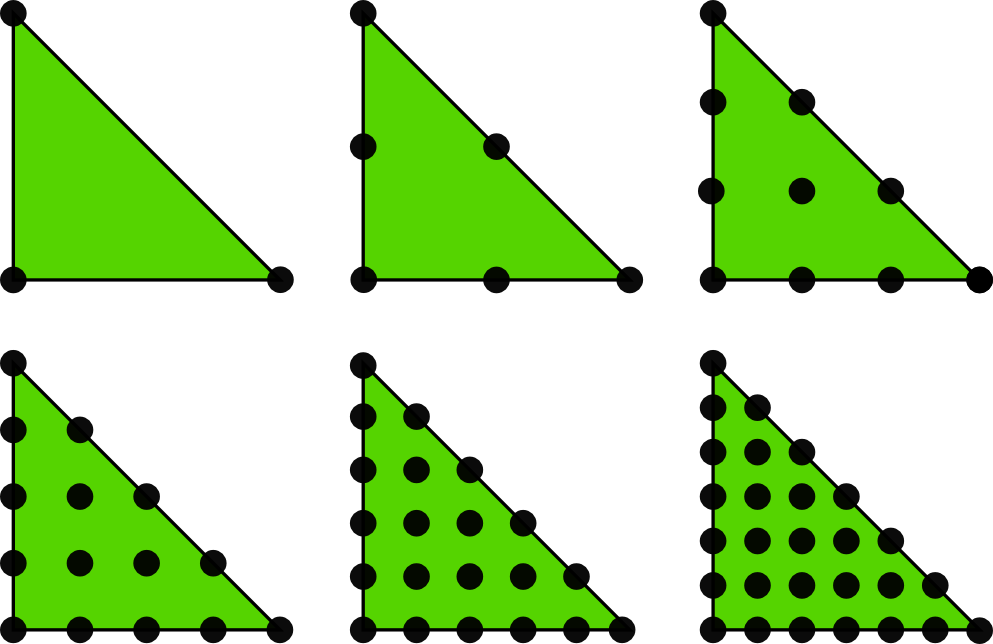
\includegraphics[width=\linewidth]{fem_triangle_2.png}
  \caption{Finite Element nodes on triangle for polynomials of different degrees}
  \label{fig:Nodes on Triangular Element}
\end{figure}

\end{itemize}

\end{frame}

%------------------------------------------------

\begin{frame}
\frametitle{Orthonormal basis function}
\begin{itemize}

\item Orthonormal basis functions are the basis functions defined in such a way that all basis functions are orthonormal to each other with respect to suitable inner product. 
\item The number of orthonormal basis functions for a given element is the same as the number of nodal basis functions. 

\begin{equation}
\begin{split}
(\hat{\phi_i } , \hat{\phi_j}) = \int_{\hat{T}} \hat{\phi_i} \hat{\phi_j} = 1 \quad \textrm{if} \quad i = j \\
(\hat{\phi_i } , \hat{\phi_j}) = \int_{\hat{T}} \hat{\phi_i} \hat{\phi_j} = 0 \quad \textrm{if} \quad i \neq j 
\end{split}
\end{equation}

\end{itemize}

\end{frame}

%------------------------------------------------



\begin{frame}
\frametitle{Conclusions}
\begin{itemize}

\item The Schur complement method is very useful for the Stokes equation due to efficient computation and good accuracy.
\item $minres$ converges slowly and $bicgstab$ does not converge
\item The condition number of the stiffness matrix of the Stokes equation increases with increase in penalty parameter. Therefore, the penalty parameter has to be small enough to limit the condition number. However, the penalty parameter has to be large enough to maintain coercivity of the bilinear form.
\item The Newton method requires solution of large system of equations in each Newton loop adding to heavy computational cost.
\item The solvers/methods which are applicable for the Saddle point problems should be used for solving the weak form of the Stokes equation.
\item The initial guess, in our case the solution obtained from the Stokes equation, is crucial for success of the Newton method.
\item The solution of the Stokes equation and the Navier Stokes equation show close to linear convergence in $L^2$ norm.
\item The higher polynomial degree does not always guarantee better accuracy. However, the convergence rate increases with increase in polynomial degree.

\end{itemize}


\end{frame}

%------------------------------------------------

\begin{frame}
\frametitle{Outlook}
\begin{itemize}

\item Test for higher Reynold's number
\item Further solvers/methods
\item Time dependent cases
\item Parametrization
\item Reduced order modelling

\end{itemize}


\end{frame}

%------------------------------------------------

\begin{frame}
\frametitle{Error definition}
\begin{itemize}

\item $h-$convergence and $p-$convergence
\begin{block}{$L^2$ error}
\begin{equation}
P_{error,L^2} = (\int_{\Omega} |P - P_h|^2)^{\frac{1}{2}} \quad \mathrm{.}
\end{equation}
\end{block}

\begin{block}{$H_0$ error}
\begin{equation}
P_{error,H_0} = \sum_{k=1}^{nel} \int_{\tau_k} |\nabla P - \nabla P_h|^2 \quad \mathrm{.}
\end{equation}
\end{block}

\end{itemize}
\end{frame}

%------------------------------------------------

\begin{frame}
\frametitle{Convergence test}

The domain considered for this example is the unit square [0,1] $\times$ [0,1] in the $x-y$ plane. 
The boundary ${x=0}$ is dirichlet boundary with inflow velocity at point $(0,y)$ as $u = (y(1-y), 0)$. The boundaries ${y = 0}$ and ${y = 1}$ are Dirichlet boundaries with no slip or zero velocity condition. The boundary ${x = 1}$ is a Neumann boundary with zero Neumann value i.e. $t = (0, 0)$. The source term is $f = (2 \nu - 1, 0)$. The analytical solution for pressure and velocity reads as,

\begin{center}

\begin{equation}
p = (1 - x)
\end{equation}

\begin{equation} 
 u = (y(1-y), 0) \quad \textrm{.}
\end{equation}

\end{center}

The results of an $h-$convergence test with velocity polynomial degree $D=2$ and pressure polynomial degree $D-1 = 2$ in the $L^2$ norm is presented in Figures \ref{fig:vel_stoke_conv}, \ref{fig:vel_stoke_conv_log}, \ref{fig:pre_stoke_conv} and \ref{fig:pre_stoke_conv_log} and in the $H_0$ semi norm is presented in Figures \ref{fig:vel_stoke_conv_h0}, \ref{fig:vel_stoke_conv_log_h0}, \ref{fig:pre_stoke_conv_h0} and \ref{fig:pre_stoke_conv_log_h0}. We see almost linear convergence in $L^2$ norm. \\

We also present results of $p-$convergence test in $L^2$ norm and $H_0$ semi norm for velocity and in $L^2$ norm for pressure (Figures \ref{p_convergence_velocity_l2}, \ref{p_convergence_velocity_h0}, \ref{p_convergence_pressure_l2}). As can be seen the higher polynomial degree does not necessarily mean more accurate solution. However, the convergence rate increases with polynomial degree and below certain step size, the higher polynomial degree provides more accurate solution.\\

\end{frame}

%------------------------------------------------

\begin{frame}
\frametitle{Lid driven cavity problem}
We next present a benchmark $CFD$ problem, the Lid-driven cavity flow \cite{Montlaur2}. We solve the Stokes flow on the unit square [0,1] $\times$ [0,1] in the $x-y$ plane. On boundaries ${x = 0}, {x = 1}$ and ${y = 0}$, we impose no slip or zero velocity Dirichlet condition. On ${y = 1}$, we impose Dirichlet condition with Dirichlet velocity,
\begin{equation}
\begin{split}
u = (10x,0) \quad \textrm{for} \quad 0 \leq x \leq 0.1 \quad \textrm{,}\\
u = (1,0) \quad \textrm{for} \quad 0.1 \leq x \leq 0.9 \quad \textrm{,}\\
u = (10 - 10x,0) \quad \textrm{for} \quad 0.9 \leq x \leq 1 \quad \textrm{.}
\end{split}
\end{equation}

The results are shown in Figures \ref{stoke_bicgstab_lid}, \ref{stoke_minres_lid} and \ref{stoke_schur_lid}. The results are found to be in agreement with literature i.e. boundary layer formation at the no slip boundaries and shape of streamline. 

\end{frame}

%------------------------------------------------
\begin{frame}
\frametitle{Lid driven cavity problem}

The domain considered for this example is the unit square [0,1] $\times$ [0,1] with a cut out cylinder of diameter 0.2 centered at $(0.5,0.5)$ i.e. the center of the cylinder coincides with the center of the square in the $x-y$ plane. The boundary ${x=0}$ is Dirichlet boundary with inflow velocity at point $(0,y)$ as $u = (y(1-y), 0)$. The boundaries ${y = 0}$ and ${y = 1}$ are Dirichlet boundaries with no slip or zero velocity condition. The boundary ${x = 1}$ is a Neumann boundary with zero Neumann value i.e. $t = (0, 0)$. The source term is $f = (0, 0)$. Figures \ref{flow_over_cylinder_bicgstab}, \ref{flow_over_cylinder_minres} and \ref{flow_over_cylinder_schur} give physically relevant result for example, low pressure zone after cylinder, high pressure zone before cylinder and wake zone after cylinder for velocity.

\end{frame}

%------------------------------------------------
\begin{frame}
\frametitle{Penalty parameter}

The condition number is measured on a unit square [0,1] $\times$ [0,1] in the $x-y$ plane with the number of intervals $10 \times 10$. We see a linear increase in the condition number of the stiffness matrix with respect to the penalty parameter (Figure \ref{effect_penalty_parameter}). The linear increase is in agreement with results of Montlaur et al. \cite{Montlaur}.

We also solve flow over cylinder problem from the section \ref{flow_over_cylinder_stokes} with penalty parameter smaller than required to maintain coercivity. The results as can be seen in Figure \ref{flow_over_cylinder_c11_low} is unable to produce physically relevant flow profile.


\end{frame}

%------------------------------------------------
\begin{frame}
\frametitle{Solver selection}

We again consider the problem from the section \ref{flow_over_cylinder_stokes}. The relative residual and the run time for the same is presented in table below.
Here, run time refers to time taken for solution of equation of form $AX = B$ and plotting.  The matrix $A$ and the vector $B$ are given in assembled form as input. Since the plotting process is exactly same, the run time compares the speed of solver or method. Relative residual is measured as $\frac{||B-AX||_2}{||B||_2}$.

\begin{Huge}
SOLVER TABLE ADD
\end{Huge}

Through the analysis of the Stokes flow, we notice that that the $bicgstab$ solver stops without converging where as the minres solver shows convergence but is slower than the Schur complement method. The Schur complement method is very fast and accurate method.

\end{frame}

%------------------------------------------------
\begin{frame}
\begin{Huge}
NAVER STOKES ADD
\end{Huge}
\end{frame}

%------------------------------------------------



\end{document} 